\documentclass{scrartcl}
\usepackage{etoolbox}
\usepackage{bbm}
\usepackage{amsmath}
\usepackage{mathabx}
\usepackage{graphicx}
\usepackage{float}
\usepackage{parskip}
\usepackage{indentfirst}
\usepackage{subfigure}
\usepackage{fancyhdr}
\pagestyle{fancy}
\setlength{\parskip}{0em}
\setlength{\parindent}{2em}

%-----------------------------------------------------------------------------
\begin{document}

%-----------------------------------------------------------------------------
% header
\lhead{Huwenbo Shi (603-778-363) shihuwenbo@ucla.edu}

% title
\newcommand*{\TitleFont}{%
      \usefont{\encodingdefault}{\rmdefault}{b}{n}%
      \fontsize{16}{20}%
      \selectfont}
\newcommand*{\AuthorFont}{%
      \usefont{\encodingdefault}{\rmdefault}{r}{n}%
      \fontsize{12}{20}%
      \selectfont}
\title{\TitleFont SoCal: supervised genotype calling via ellipsoidal
separation for Affymetrix SNP microarray}
\author{\AuthorFont Huwenbo Shi (603-778-363) shihuwenbo@ucla.edu}
\date{}
\maketitle
%-----------------------------------------------------------------------------


%-----------------------------------------------------------------------------
% introduction
\section{Introduction}

\par
% background
SNP microarray is a cost--effective approach to genotype samples for specific
association studies. % cite
In Affymetrix SNP microarrays, oligonucleotide probes are first used to bind
DNA fragments containing SNPs. % cite
Then, for each SNP, a fluorescence scanner quantifies perfect match (PM) and
mismatch (MM) for each of the two alleles, denoted by A and B, on
each strand of the DNA fragment. %cite
The genotype calling procedure for SNP microarray consists of two steps.
In the first step, information from microarray is summarized to obtain the
intensities, $\theta_A$ and $\theta_B$, of the two alleles of each SNP.
In the second step, SNPs are classified into genotype AA, AB, or BB based on
the allele intensities they generate.
The focus of this article is on the second step of the genotype calling
procedure---genotype classification using summarized allele intensities.

\par
% specific background
For a specific SNP, if a sample has genotype AA or BB, the intensity,
$\theta_A$ or $\theta_B$, will be higher respectively. 
If a sample has genotype AB, the intensities, $\theta_A$ and $\theta_B$,
will be similar.
If one plots $log(\theta_A)$ versus $log(\theta_B)$ of a SNP for a number of
samples, normally 3 ellipsoidal clusters are observed, one for each genotype,
as shown in Figure \ref{fig:intro_genclus}.
Many genotype calling algorithms use model--based unsupervised clustering
methods to identify clusters and then assign genotypes to each cluster.
To estimate model parameters, these methods use the EM algorithm, which is
sensitive to starting parameters and slow to converge.
Rabbee et al. proposed the RLMM algorithm, a supervised genotype calling
method that uses reference genotype calls to form Gaussian decision
boundaries for each genotype.
This method involves fitting a linear mixed model, which can be computationally
intensive.

\par
% problem
As the number of probes on SNP microarrays and the number of individuals involved
in association studies continue to increase, both fast and accurate genotype
calling algorithms are needed.

% intro genotype cluster figure
\begin{figure}[H]
\centering
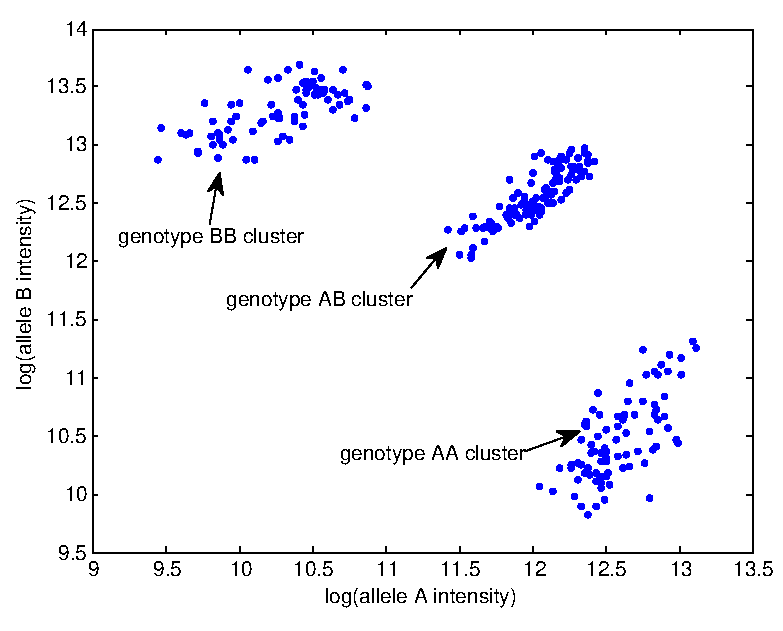
\includegraphics[scale=0.75]{intro_figs/intro_genotype_clusters.pdf}
\caption{Genotype clusters obtained from Affymetrix SNP array
allele intensity values}
\label{fig:intro_genclus}
\end{figure}

%-----------------------------------------------------------------------------









%-----------------------------------------------------------------------------
% method
\section{Method}

% overview of method
\par
SNP allele intensities are first summarized from raw microarray data using
SNPRMA.
After this step, SoCal calls genotypes in two steps.
In the first step, SoCal finds ellipsoidal regions containing each of the
genotype of a SNP using reference genotype calls.
In the second step, SoCal classifies samples with unknown genotypes using
minimum distance classification.

\par
The organization of this seciton is as follows.
First, I introduce the problem of pattern separation by ellipsoids and how
SoCal forms ellipsoidal region for each genotype of a SNP.
Then, I show how SoCal uses these ellipsoids to call genotypes.

\subsection{Pattern separation by ellipsoids}

\par
Talk about ellipsoidal separation

\subsection{Missing clusters}
Talk about how SoCal handles missing clusters

\subsection{Genotype calling and outlier detection}
Talk about how classification and outlier detection is done

%-----------------------------------------------------------------------------

\end{document}
